\section{Build Automation}

\begin{mdframed}
    \textbf{Build automation:} processo di automazione della creazione di una software build e dei processi associati, tra cui la compilazione del codice sorgente del computer in codice binario, il confezionamento del codice binario e l'esecuzione di test automatici.
\end{mdframed}
\begin{itemize}
    \item \textbf{Build-automation utility:} whose primary purpose is to generate build artifacts through activities like compiling and linking source code.
    \begin{itemize}
        \item scripting tools: \verb|.sh|, \verb|.bat|, \verb|Makefile|, Gradle, ...
        \item artifact oriented tools: Apache Maven, ...
    \end{itemize}
    \item \textbf{Build-automation server:} strumenti generali web based che eseguono utilità di build-automation su base programmata o attivata.
\end{itemize}

\subsection{Processo di Build}
\begin{mdframed}
    \textbf{Processo di build:} insieme di passi che trasformano gli script di build, il codice sorgente, i file di configurazione, la documentazione e i test in un prodotto software distribuibile.
\end{mdframed}
\begin{center}
    \begin{tabular}{c}
        \\ 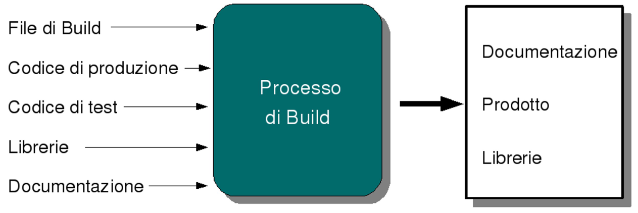
\includegraphics[width=0.9\textwidth]{images/Build1.png} \\ \\
    \end{tabular}
\end{center}

\subsubsection{Caratteristiche CRISP}
\begin{itemize}
    \item \textbf{Completo:} Indipendente da fonti non specificate nello script di build
    \item \textbf{Ripetibile:} Accede ai file contenuti nel sistema di gestione del codice sorgente. Una esecuzione ripetuta dà lo stesso risultato
    \item \textbf{Informativo:} Fornisce informazioni sullo stato del prodotto
    \item \textbf{Schedulabile:} Può essere programmato ad una certa ora e fatto eseguire automaticamente
    \item \textbf{Portabile:} Indipendente il più possibile dall’ambiente di esecuzione
\end{itemize}

\newpage
\subsection{Maven}
\begin{mdframed}
    Apache Maven: strumento di gestione e comprensione dei progetti software. Basato sul concetto di \textbf{Project Object Model (POM)}, Maven è in grado di gestire la compilazione, la reportistica e la documentazione di un progetto da un'informazione centrale.
\end{mdframed}

\subsubsection{Caratteristiche}
\begin{itemize}
    \item \textbf{Build Tool:} sono definite delle Build Lifecycle che permettono di configurare ed eseguire il processo di build.
    \item \textbf{Dependency Management:} Le dipendenze di progetto vengono specificate nel file di configurazione \verb|pom.xml|. Maven si occupa di scaricarle in automatico da dei Repository remoti e salvarle in un repository locale.
    \item \textbf{Remote Repositories:} sono stati definiti dei repository remoti dove sono presenti gran parte delle librerie di progetti opensource e dei plugin utilizzati da maven per implementare e estendere le fasi dei Build Lifecycle
    \item \textbf{Universal Reuse of Build Logic:} Le Build Lifecycle, i plugin Maven permettono di definire in modo riusabile i principali aspetti richiesti per la gestione di progetto. Tra cui: l'esecuzione del processo di build, l'esecuzione di framework di test (Junit/TestNG), la creazione di template di progetto.
\end{itemize}

\subsubsection{Build Lifecycle}
Esistono 3 Build Lifecycles:
\begin{itemize}
    \item \textbf{Default Lifecycle:} gestisce la distribuzione del progetto.
    \item \textbf{Clean Lifecycle:} gestisce la pulizia del progetto.
    \item \textbf{Site Lifecycle:} gestisce la creazione della documentazione del sito del progetto.
\end{itemize}
La Default Build Lifecycle è composta dalle seguenti fasi:
\begin{enumerate}
    \item \textbf{Validate:} convalidare la correttezza del progetto e la disponibilità di tutte le info necessarie.
    \item \textbf{Compile:} compilare il codice sorgente del progetto.
    \item \textbf{Test:} testare il codice sorgente compilato utilizzando un framework di unit testing adeguato.
    \item \textbf{Package:} prendere il codice compilato e confezionarlo nel suo formato distribuibile (e. \verb|JAR|).
    \item \textbf{Verify:} eseguire eventuali controlli sui risultati dei test di integrazione per garantire il rispetto dei criteri di qualità.
    \item \textbf{Install:} installa il pacchetto nel repository locale, per utilizzarlo come dipendenza in altri progetti a livello locale.
    \item \textbf{Deploy:} eseguito nell'ambiente di compilazione, copia il pacchetto finale nel repository remoto per condividerlo con altri sviluppatori e progetti.
\end{enumerate}

\newpage
\subsection{POM}
\begin{mdframed}
    \textbf{Project Object Model:} unità di lavoro fondamentale in Maven. È un file \verb|XML| che contiene informazioni sul progetto e dettagli di configurazione usati da Maven per costruire il progetto.
\end{mdframed}
Alcune delle configurazioni che possono essere specificate nel POM sono:
\begin{itemize}
    \item Project dependencies
    \item Plugin o goals che possono essere eseguiti
    \item Build profiles
    \item Altre info come: project version, description, developers, ...
    \item Project ID (group ID + artifact ID + version)
\end{itemize}

\subsubsection{Project Archetypes}
In breve, Archetype è un toolkit di template per progetti Maven. Un archetipo è definito come un modello o uno schema originale da cui si ricavano tutte le altre cose dello stesso tipo. \\
Il nome si adatta al fatto che stiamo cercando di fornire un sistema che fornisca un mezzo coerente per generare progetti Maven. \\
Archetype aiuterà gli autori a creare modelli di progetti Maven per gli utenti e fornirà agli utenti i mezzi per generare versioni parametrizzate di tali modelli di progetto.

\subsubsection{Maven Plugin}
Maven è un framework di base per un insieme di plugin Maven. I plugin vengono utilizzati per:
\begin{itemize}
    \item Creare file \verb|jar|
    \item Creare file \verb|war|
    \item Compilare codice
    \item Codicec di Unit Test
    \item Creare Project Documentation
\end{itemize}
Quasi tutte le azioni che si possono pensare di eseguire su un progetto sono implementate come plugin Maven.

\newpage